\PassOptionsToPackage{svgnames, table}{xcolor}
\documentclass[8pt]{extarticle}
\usepackage[spanish,es-nodecimaldot]{babel}

\usepackage{mcs_style}

\usepackage{bm}
\usepackage{comment}
\usepackage{fontawesome}

% Usaremos \cmdo{} para el estilo del comando

\newcommand{\cmdo}[1]{\texttt{\small\bfseries#1}} %boldface truewriter Fira Mono
\newcommand{\cmdoesp}[1]{\texttt{\small\bfseries\detokenize{#1}}} %comando especial para cuando el comando contenga simbolos sensibles en Latex (p.ej. ^, \,...)

\newcommand{\up}[1]{${}^\mathrm{#1}$}

\newcommand{\hseparador}{\chline{gray!50!Header}}
\newcommand{\hlinefinal}{\chline{Header}\chline{Header}}
\newcommand{\hseparadorAlt}{\chline{gray!50!HeaderAlt}}
\newcommand{\hlinefinalAlt}{\chline{HeaderAlt}\chline{HeaderAlt}}


\begin{document}
    
    \fullwidthheader{Matlab/Octave:\,\,Bestiario\,\,de\,\,comandos\,\,y\,\,sentencias}
    %\fullwidthheader{MATLAB\,\,CHEAT\,\,SHEET}
    
    \begin{center}
        \vspace*{0.5cm}
        {\Large\bfseries A lo largo de este documento, $\bm{x}$ e $\bm{y}$ ser\'an vectores fila o columna, $\bm{z}$ un n\'umero complejo, y $\bm{A}$ una matriz.}
    \end{center}
    
    \begin{multicols}{3}
        \centering
        
        % -------------------------------------------------------
        % Espacio de trabajo: basicos
        % -------------------------------------------------------
        \begin{fancytable}{Espacio de trabajo: b\'asicos}
            \cmdo{Ctrl + C} & Aborta la operaci\'on o sentencia actual en la l\'inea de comandos\\
            \hseparador%
            \cmdo{clc} & Limpia la ventana de comandos\\
            \cmdo{clear} & Borra todas las variables\\
            \cmdo{clear x A} & Borra las variables $x$ y $A$\\
            \hseparador%
%             \cmdo{format short} & Muestra n\up{os} con 4 decimales\\
%             \cmdo{format short e} & Muestra n\up{os} con 4 decimales en notaci\'on exponencial\\
%             \cmdo{format long} & Muestra n\up{os} con 15 decimales\\
%             \cmdo{format long e} & Muestra n\up{os} con 15 decimales en notaci\'on exponencial\\
%             \cmdo{format rat} & Muestra n\up{os} en formato racional\\
%             \hseparador%
            \cmdo{diary 'fichero.txt'} & Registra en un fichero lo que se hace en la ventana de comandos\\
            \cmdo{diary off} & Para el registro\\
            \cmdo{diary on} & Reanuda el registro\\
            \hseparador%
            \cmdo{save fichero} & Guarda las variables definidas en el fichero\\
            \cmdo{save fichero x A} & Guarda las variables $x$ y $A$ en el fichero\\
            \cmdo{load fichero} & Carga las variables almacenadas en el fichero\\
            \hseparador%
%             \cmdo{clf} & Clear all plots\\
%             \cmdo{close all} & Close all plots\\
%             \hseparador%
%             \cmdo{doc comando} & Abre la ayuda del comando\\
            \cmdo{pwd} & Muestra la ubicaci\'on del directorio de trabajo actual\\
            \cmdo{dir} & Muestra el contenido del directorio de trabajo actual\\
            \cmdo{cd carpeta} & Permite acceder a una carpeta del directorio de trabajo actual \\
            \hseparador%
            \cmdo{help comando} & Abre la documentaci\'on del comando\\
            \cmdo{lookfor 'texto'} & Busca el texto en la documentaci\'on de comandos\\
            \hseparador%
            \cmdo{...} & Conecta una misma sentencia escrita en dos lineas seguidas de c\'odigo\\
            \cmdo{comando;} & La ``\cmdo{;}'' suprime la salida del comando\\
            \cmdo{nombreprograma} & Ejecuta \emph{nombreprograma.m}\\
            \cmdo{tic, sentencias, toc} & Devuelve el tiempo de ejecuci\'on total de las sentencias\\
%             \hseparador%
%             \cmdo{\%Esto es un comentario} & Comentarios\\
%             \cmdo{disp('texto')} & Muestra el texto\\
%             \cmdo{disp(x)} & Muestra la variable $x$\\
            \hlinefinal%
        \end{fancytable}

        % -------------------------------------------------------
        % Espacio de trabajo: formato y salida
        % -------------------------------------------------------
        \begin{fancytableAlt}{Espacio de trabajo: formato y salida}
            \cmdo{format short} & Muestra n\up{os} con 4 decimales\\
            \cmdo{format short e} & Muestra n\up{os} con 4 decimales en notaci\'on exponencial\\
            \cmdo{format long} & Muestra n\up{os} con 15 decimales\\
            \cmdo{format long e} & Muestra n\up{os} con 15 decimales en notaci\'on exponencial\\
            \cmdo{format rat} & Muestra n\up{os} en formato racional\\
            \hseparadorAlt%
            \cmdo{\% Esto es un comentario} & Comentarios\\
            \cmdo{disp('texto')} & Muestra el texto\\
            \cmdo{disp(x)} & Muestra el contenido de la variable $x$\\
            \hlinefinalAlt
        \end{fancytableAlt}

        
        % -------------------------------------------------------
        % Constantes
        % -------------------------------------------------------
        \begin{fancytable}{Constantes num\'ericas}
            \cmdo{pi} & $\pi\simeq 3.1415926535897$\\
            \cmdo{i} \'o \cmdo{j} & Unidad imaginaria $\sqrt{-1}$\\
            \cmdo{Inf} & Infinito\\
            \cmdo{NaN} & ``No es un n\'umero'' (p.ej., $0/0$) \\
            \cmdo{eps} & Precisión relativa de m\'aquina en doble precisi\'on (por defecto, $2.2204\cdot 10^{-16}$) \\
            \cmdo{realmax} & Nº positivo m\'as grande en doble precisi\'on, $1.7977\cdot 10^{308}$\\
            \cmdo{realmin}~~~~~~~~~~ & Nº positivo m\'as peque\~no en doble precisi\'on $2.2251\cdot 10^{-308}$\\
            \hlinefinal%
        \end{fancytable}

        % -------------------------------------------------------
        % Operaciones aritm\'eticas y funciones b\'asicas
        % -------------------------------------------------------
        \begin{fancytable}{Operaciones aritm\'eticas y funciones b\'asicas}
            \cmdo{1.349} & Los decimales de un real se definen CON EL PUNTO {\bf ``.''} NO con comas o tildes \\
            \cmdo{3+4}, \cmdo{7*4}, \cmdo{2-6}~~~~~~~~~& Suma, producto y resta \\
            \cmdo{8/3}, \cmdoesp{3\8} & Divisi\'on por la derecha y por la izquierda \\
            \cmdoesp{3^7} & Calcula la potencia $3^7$\\
            \cmdo{rem(17,3)} & Resto de la divisi\'on de $17$ entre $3$ \\
            \hseparador%
            \cmdo{sqrt(5)} & Calcula la ra\'iz cuadrada $\sqrt{5}$\\
            \cmdo{log(3)} & Calcula el logaritmo neperiano $\ln(3)$\\
            \cmdo{log10(100)} & Calcula el logaritmo $\log_{10}(100)$\\
            \cmdo{abs(-5)} &  Calcula el valor absoluto $|-5|$\\
            \cmdo{sin(5*pi/3)} & Calcula el seno $\sin(5\pi/3)$\\
            \cmdo{cos(-pi/3)} & Calcula el coseno $\cos(-\pi/3)$\\
            \cmdo{exp(3)} & Calcula la exponencial $e^3$\\
%             \cmdo{floor(3.8)} & Compute $\left \lfloor 3.8 \right \rfloor$\\
            \hlinefinal%
        \end{fancytable}

        % -------------------------------------------------------
        % N\'umeros complejos
        % -------------------------------------------------------
        \begin{fancytable}{N\'umeros complejos}
            \hspace*{-1.5ex}$\begin{array}{l}\text{\cmdo{z=1-2*i}~~~\'o}\\ \text{\cmdo{z=complex(1,-2)}} \end{array}$
            & Crea el n\'umero complejo $z=1-2i$\newline (a partir de las partes real e imaginaria)\\
            \cmdo{abs(z)} & M\'odulo (valor absoluto) de $z$ \\
            \cmdo{angle(z)} & Argumento de $z$ \\
            \cmdo{z'} & Conjugado de $z$ \\
            \cmdo{real(z)} & Parte real de $z$ \\
            \cmdo{imag(z)} & Parte imaginaria de $z$ \\
            \cmdo{isreal(z)} & Devuelve 1 si $z$ es real, 0 si no \\
            \hlinefinal%
        \end{fancytable}

        % -------------------------------------------------------
        % Definiendo variables b\'asicas
        % -------------------------------------------------------
        \begin{fancytable}{Definiendo variables b\'asicas}
            \cmdo{a = 3} & Define la variable $a$ como $3$\\
            \cmdo{b = 4.321} & Define la variable $b$ como $4.321$\\
            \cmdo{c = 'texto'} & Define en $c$ una cadena de caracteres con el texto \\
            \cmdo{cond = logical(1)} & Define en $cond$ el valor l\'ogico 1 (\emph{true}) \\
            \hlinefinal
        \end{fancytable}

        % -------------------------------------------------------
        % Ejemplo: valores l\'ogicos
        % -------------------------------------------------------
        \begin{exampleBlock}{Ejemplo: valores l\'ogicos y operaciones}
            \matlabcode{MatlabFiles/logic.m}
        \end{exampleBlock}


        % -------------------------------------------------------
        % Vectores y matrices: generaci\'on y acceso
        % -------------------------------------------------------
        \begin{fancytable}{Vectores y matrices: generaci\'on y acceso}
            \cmdo{x = [1, 2, 3]}~~~\'o & Define $x$ como el vector \\
            \rowcolor{row1!75}
            \cmdo{x = [1 2 3]} &  fila $[1, 2, 3]$\\
            \rowcolor{row1!0}
            \cmdo{x = [1; 2; 3]}~~~\'o & Define $x$ como el vector\\
            \cmdo{x = [1, 2, 3]'} &  columna $[1, 2, 3]^{t}$ \\
            \cmdo{7:15} & Vector fila con $7,\,8,\ldots,14,\,15$ \\
            \cmdo{1.1:0.2:3.3} & Vector fila con $1.1,\,1.3,\ldots,3.3$ \\
            \cmdo{linspace(2, 6.5, 100)} & Genera un vector fila con $100$ componentes equiespaciadas entre el $2$ y el $6.3$\\
            \cmdo{A = [1, 2, 3, 4;} &  \\
            \rowcolor{row1!0}\qquad\,\,\,\cmdo{5, 6, 7, 8;} & Define $A$ como una matriz $3 \times 4$ \\
            \qquad\,\,\,\cmdo{9, 10, 11, 12]} & \\
%             \hseparador%
%             \cmdo{x(2) = 7} & Change $x$ from $[1, 2, 3]$ to $[1, 7, 3]$\\
%             \cmdo{A(2,1) = 0} & Change $A_{2,1}$ from $5$ to $0$ \\
            \hseparador%
            \cmdo{x(2:12)} & Del 2\up{o}  al 12\up{o} elemento de $x$\\
            \cmdo{x(2:end)} & Del 2\up{o}  al \'ultimo elemento de $x$\\
            \cmdo{x(1:2:end)} & El 1\up{er}, 3\up{er}, 5\up{o},...hasta el \'ultimo elemento de $x$.\\
            \cmdo{A(3,4)} & El elemento de la 3\up{a} fila y la 4\up{a} columna de $A$\\
            \cmdo{A(3,:)} & La 3\up{a} fila de $A$\\
            \cmdo{A(:,4)} & La 4\up{a} columna de $A$\\
            \cmdo{A(2, 1:5)} & Del 1\up{o} al 5\up{o} elemento de la 2\up{a} fila \\
            \cmdo{A([1,3],4)} & Los elementos de la 1\up{a} y 3\up{a} fila que se encuentran en la 4\up{a} columna \\
            \hseparador%
            \cmdo{A(:)} & La matriz $A$ vista como vector columna (con los elementos en orden columna)\\
%             \cmdo{A(7)} & El 7\up{o} elemento del vector columna \cmdo{A(:)} \\
            \hlinefinal
        \end{fancytable}

    \end{multicols}

    \newpage

    \fullwidthheader{Matlab/Octave:\,\,Bestiario\,\,de\,\,comandos\,\,y\,\,sentencias}
    %\fullwidthheader{MATLAB\,\,CHEAT\,\,SHEET}

    \vspace*{0.5cm}

%     \begin{center}
%         \vspace*{0.5cm}
%         {\Large\bfseries A lo largo de este documento, $\bm{x}$ e $\bm{y}$ ser\'an vectores fila o columna, $\bm{z}$ un n\'umero complejo, y $\bm{A}$ una matriz.}
%     \end{center}

    \begin{multicols}{3}
        \centering
        
        % -------------------------------------------------------
        % Vectores y matrices: composici\'on y borrado
        % -------------------------------------------------------
        \begin{fancytable}{Vectores y matrices: composici\'on y borrado}
            \cmdo{[A ; B]} & Matriz compuesta por las filas de $A$ sobre las filas de $B$ (con mismo n\up{o} de columnas)\\
            \cmdo{[A , B]} & Matriz compuesta por las columnas de $A$ seguidas de las de $B$ (con mismo n\up{o} de filas)\\
            \cmdo{[3,v; c d]} & Matriz compuesta por 3 seguido de la fila de $v$, sobre las columnas de $c$ seguidas de las de $d$\\
            \hseparador%
            \cmdo{A = []} & Borra todos los elementos de $A$ \\
            \cmdo{x(4) = []} & Elimina la 4\up{a} componente de $x$ \\
            \cmdo{A(3,:) = []} & Elimina la 3\up{a} fila $A$ \\
            \hlinefinal%
        \end{fancytable}


        % -------------------------------------------------------
        % Operaciones de vectores y matrices
        % -------------------------------------------------------
        \begin{fancytable}{Operaciones de vectores y matrices}
            \cmdo{3 * x} & Multiplica cada elemento de $x$ por $3$\\
            \cmdo{x + 2} & Suma $2$ a cada elemento de $x$\\
            \cmdo{x + y} & Suma elemento a elemento los vectores $x$ e $y$\\
            \cmdo{A * y} & Producto de una matriz y un vector\\
            \cmdo{A * B} & Producto (matricial) de dos matrices $A\cdot B$\\
            \cmdo{A .* B} & Producto (elemento a elemento) de dos matrices\\
            \cmdoesp{A ^ 3} & La matriz (cuadrada) $A$ elevada a la 3\up{a} potencia\\
            \cmdoesp{A .^ 3} & La matriz con los elementos de $A$ elevados a la 3\up{a} potencia\\
            \cmdo{A'} & Traspuesta de $A$\\
            \cmdo{inv(A)} & Inversa de $A$\\
            \cmdo{A / 3} & Divide cada elemento de $A$ por $3$ \\
            \cmdo{3 ./ A} & Devuelve la matriz donde cada elemento es $3$ dividido por el correspondiente de $A$ \\
            \cmdo{A / B} & Devuelve $A\cdot B^{-1}$\\
            \cmdoesp{A \ B} & Devuelve $A^{-1}\cdot B$\\
            \cmdo{A ./ B} & Divisi\'on (elemento a elemento) de dos matrices\\
            \hlinefinal%
        \end{fancytable}

        % -------------------------------------------------------
        % Funciones auxiliares de vectores y matrices
        % -------------------------------------------------------
        \begin{fancytable}{Funciones auxiliares de vectores y matrices}
            \cmdo{length(x)} & N\up{o} de componentes de $x$ \\
            \cmdo{size(A)} & Tama\~no de $A$ \\
            \cmdo{[m,n]=size(A)} & Asigna a $m$ el n\up{o} de filas y a $n$ el n\up{o} de columnas de $A$ \\
            \cmdo{sum(x)} & Suma todos los elementos de $x$\\
            \cmdo{sum(A)} & Vector de sumas de cada columna de $A$\\
            \cmdo{prod(x)} & Multiplica todos los elementos de $x$\\
            \cmdo{prod(A)} & Vector de productos de cada columna de $A$\\
            \cmdo{sort(x)} & Ordena ascendentemente los elementos de $x$\\
            \cmdo{sort(A)} & Ordena ascendentemente de forma independiente cada columna de $A$\\
            \cmdo{max(x)} & Valor m\'aximo de $x$\\
            \cmdo{max(A)} & Vector con el m\'aximo de cada columna de $A$\\
            \cmdo{min(x)} & Valor m\'inimo de $x$\\
            \cmdo{min(A)} & Vector con el m\'inimo de cada columna de $A$\\
            \hlinefinal%
        \end{fancytable}


        % -------------------------------------------------------
        % Ejemplo: estructura b\'asica de un programa
        % -------------------------------------------------------
        \begin{exampleBlock}{Ejemplo: estructura b\'asica de un programa}
            \matlabcode{MatlabFiles/programa.m}
        \end{exampleBlock}

        % -------------------------------------------------------
        % Entrada y salida de datos
        % -------------------------------------------------------
        \begin{fancytableAlt}{Entrada y salida de datos}
            \cmdo{a=input('Introduce dato:')} & Saca en pantalla el texto de entrada de dato y se lo asigna a $a$ al presionar {\bf Enter} \\
            \cmdo{c=input('?`Nombre?','s')} & Asigna la cadena de caracteres introducida por usuario  \\
            \hseparadorAlt%
            \cmdo{disp(A)}~~\'o~~\cmdo{disp('texto')} & Muestra $A$ o texto \\
            \cmdo{fprintf('Es a=\%f \cmdoesp{\n}', a)} & Escribe en pantalla el texto combinado con el dato de $a$ \\
            \cmdo{c=sprintf('Es a=\%f \cmdoesp{\n}', a)} & Almacena en $c$ la cadena de caracteres del texto combinado con el dato de $a$ \\
%             \hseparadorAlt%
%             \cmdo{\%f} & Formato de salida de datos en coma flotante \\
%             \cmdo{\%d} & Formato de salida de datos como enteros, l\'ogicos,... \\
%             \cmdo{\%s} & Formato de salida de cadenas de caracteres \\
%             \hseparadorAlt%
%             \cmdo{\%-6.3f} & Salida de datos, justificado a izqda, con 6 caracteres reservados para salida \\
%             \cmdo{\%d} & Formato de salida de datos como enteros, l\'ogicos,... \\
%             \cmdo{\%s} & Formato de salida de cadenas de caracteres \\
            \hlinefinalAlt%
        \end{fancytableAlt}

        % -------------------------------------------------------
        % Formato de salida de datos
        % -------------------------------------------------------
        \begin{fancytableAlt}{Formato de salida de datos}
            \cmdo{\%f} & Formato en coma flotante (escribe con 6 decimales) \\
            \cmdo{\%d} & Formato como enteros, l\'ogicos,... \\
            \cmdo{\%s} & Formato de cadenas de caracteres \\
            \hseparadorAlt%
            \cmdo{\%-6.3f} & Salida de datos en coma flotante, justificado a izqda. (con \cmdo{-}), con 6 caracteres m\'inimos reservados para escritura, escrito con 3 decimales \\
            \cmdo{\%4.2d} & Salida de datos de enteros etc, justificado a dcha. (sin \cmdo{-}), con 4 caracteres m\'inimos reservados para escritura, con un m\'inimo de 2 d\'igitos \\
            \cmdo{\%7s} & Salida de cadenas de caracteres, justificado a dcha. (sin \cmdo{-}) con m\'inimo de anchura de 7 caracteres \\
            \hlinefinalAlt%
        \end{fancytableAlt}

        % -------------------------------------------------------
        % Generaci\'on de elementos aleatorios
        % -------------------------------------------------------
        \begin{fancytable}{Generaci\'on de elementos aleatorios}
            \cmdo{rand()} & Genera n\up{o} aleatorio equiprobable en el intervalo ABIERTO $(0,1)$ \\
            \cmdo{rand(3)} & Genera una matriz $3\times 3$ de n\up{os} aleatorios equiprobables en $(0,1)$ \\
            \cmdo{rand(4,2)} & Genera una matriz $4\times 2$ de reales aleatorios equiprobables en $(0,1)$ \\
            \cmdo{2+13*rand()} & Genera n\up{o} aleatorio equiprobable en $(2,15)$ \\
            \cmdo{fix(1+6*rand())} & Genera n\up{o} ENTERO aleatorio equiprobable en el intervalo CERRADO $[1,6]$\\
            \hlinefinal%
        \end{fancytable}
        
        % -------------------------------------------------------
        % Ejemplos: Sentencias condicionales
        % -------------------------------------------------------
        \begin{exampleBlock}{Ejemplos: Sentencias condicionales}
            \matlabcode{MatlabFiles/ifelseifelse.m}
        \end{exampleBlock}


        % -------------------------------------------------------
        % Ejemplos: Bucles for I
        % --------------------------------------------\normalsize-----------
        \begin{exampleBlock}{Ejemplos: Bucle for {\small (I)} }
        \matlabcode{MatlabFiles/forloop.m}
        \end{exampleBlock}

        % -------------------------------------------------------
        % Ejemplos: Bucles for II
        % -------------------------------------------------------
        \begin{exampleBlock}{Ejemplos: Bucle for {\normalsize (III)} }
        \matlabcode{MatlabFiles/forloop2.m}
        \end{exampleBlock}

        % -------------------------------------------------------
        % Ejemplos: Bucles for III
        % -------------------------------------------------------
        \begin{exampleBlock}{Ejemplos: Bucle for {\normalsize (III)} }
        \matlabcode{MatlabFiles/forloop3.m}
        \end{exampleBlock}

        % -------------------------------------------------------
        % Ejemplos: Bucles while I
        % -------------------------------------------------------
        \begin{exampleBlock}{Ejemplos: Bucle while {\normalsize (I)} }
            \matlabcode{MatlabFiles/whileLoop.m}
        \end{exampleBlock}

        % -------------------------------------------------------
        % Ejemplos: Bucles while II
        % -------------------------------------------------------
        \begin{exampleBlock}{Ejemplos: Bucle while {\normalsize (II)} }
            \matlabcode{MatlabFiles/whileLoop2.m}
        \end{exampleBlock}

    \end{multicols}

     \begin{comment}

    \newpage

    \fullwidthheader{Matlab/Octave:\,\,Bestiario\,\,de\,\,comandos}
    %\fullwidthheader{MATLAB\,\,CHEAT\,\,SHEET}

    \vspace*{0.5cm}

    \begin{multicols}{3}
        \centering

        % -------------------------------------------------------
        % Ejemplos: Bucle for anidado I
        % -------------------------------------------------------
        \begin{exampleBlock}{Ejemplos: Bucle for anidado I}
        \matlabcode{MatlabFiles/foranidado.m}
        \end{exampleBlock}

        % -------------------------------------------------------
        % Ejemplos: Bucle for anidado II
        % -------------------------------------------------------
        \begin{exampleBlock}{Ejemplos: Bucle for anidado II}
        \matlabcode{MatlabFiles/foranidado2.m}
        \end{exampleBlock}

        % -------------------------------------------------------
        % Ejemplos: Bucle while para condici\'on input
        % -------------------------------------------------------
        \begin{exampleBlock}{Ejemplos: Bucle while para condici\'on input}
        \matlabcode{MatlabFiles/foranidado.m}
        \end{exampleBlock}
        

    \end{multicols}
    
    \newpage

    \fullwidthheader{Matlab/Octave:\,\,Bestiario\,\,de\,\,comandos}
    %\fullwidthheader{MATLAB\,\,CHEAT\,\,SHEET}

    \vspace*{0.5cm}

    \begin{multicols}{3}
        \centering

        % -------------------------------------------------------
        % Ejemplos: Bucle for anidado I
        % -------------------------------------------------------
        \begin{exampleBlock}{Ejemplos: Bucle for anidado I}
        \matlabcode{MatlabFiles/foranidado.m}
        \end{exampleBlock}

        % -------------------------------------------------------
        % Ejemplos: Bucle for anidado II
        % -------------------------------------------------------
        \begin{exampleBlock}{Ejemplos: Bucle for anidado II}
        \matlabcode{MatlabFiles/foranidado2.m}
        \end{exampleBlock}

        % -------------------------------------------------------
        % Ejemplos: Bucle while para condici\'on input
        % -------------------------------------------------------
        \begin{exampleBlock}{Ejemplos: Bucle while para condici\'on input}
        \matlabcode{MatlabFiles/foranidado.m}
        \end{exampleBlock}

        % -------------------------------------------------------
        % Ejemplos: Bucle for anidado II
        % -------------------------------------------------------
        \begin{exampleBlock}{Ejemplos: Bucle for anidado II}
        \matlabcode{MatlabFiles/foranidado2.m}
        \end{exampleBlock}


        % -------------------------------------------------------
        % Constructing Matrices/Vectors
        % -------------------------------------------------------
        \begin{fancytable}{Constructing Matrices and Vectors}
            \cmdo{zeros(12, 5)} & Make a $12 \times 5$ matrix of zeros\\
            \cmdo{ones(12, 5)} & Make a $12 \times 5$ matrix of ones\\
            \cmdo{eye(5)} & Make a $5 \times 5$ identity matrix\\
            \cmdo{eye(12, 5)} & Make a $12 \times 5$ identity matrix\\
            \hlinefinal%
        \end{fancytable}

        % -------------------------------------------------------
        % Plotting
        % -------------------------------------------------------
        \begin{fancytable}{Plotting}
            \cmdo{plot(x,y)} & Plot $y$ versus $x$ (must be the same length)\\
            \cmdo{loglog(x,y)} & Plot $y$ versus $x$ on a log-log scale (both axes have a logarithmic scale)\\
            \cmdo{semilogx(x, y)} & Plot $y$ versus $x$ with $x$ on a log scale\\
            \cmdo{semilogy(x, y)} & Plot $y$ versus $x$ with $y$ on a log scale\\
            \cmdo{axis equal} & Force the $x$ and $y$ axes to be scaled equally\\
            \cmdo{title('A Title')} & Add a title to the plot\\
            \cmdo{xlabel('x label')} & Add a label to the $x$ axis\\
            \cmdo{ylabel('y label')} & Add a label to the $y$ axis\\
            \cmdo{legend('foo', 'bar')} & Label 2 curves for the plot\\
            \cmdo{grid} & Add a grid to the plot\\
            \cmdo{hold on} & Multiple plots on single figure\\
            %\cmdo{axis([xmin, xmax,\newline \hspace*{0.86cm}ymin, ymax])} & Set the view for the plot\\
            \cmdo{figure} & Start a new plot\\
            \hlinefinal%
        \end{fancytable}


        % Functions
        \begin{exampleBlock}{Funciones}
            \matlabcode{MatlabFiles/functions.m}
        \end{exampleBlock}

        % Function handles
        \begin{exampleBlock}{Funciones abreviadas}
            \matlabcode{MatlabFiles/functionHandles.m}
        \end{exampleBlock}

        % Plotting
        \begin{exampleBlock}{Gr\'aficas}
            \matlabcode{MatlabFiles/plotting.m}%
            \quad\\

            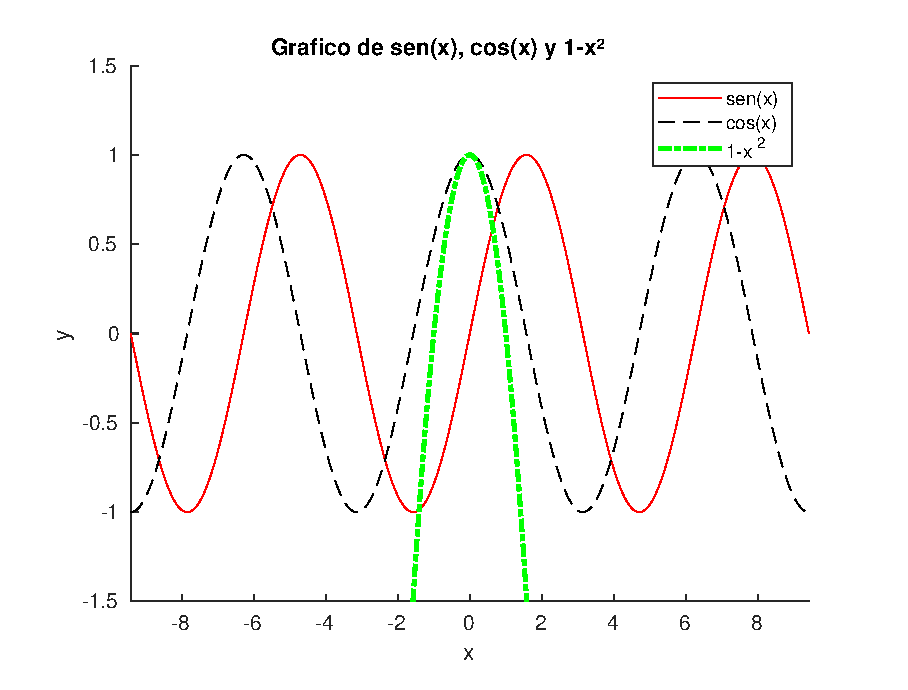
\includegraphics[width=\textwidth]{plotting.eps}
        \end{exampleBlock}

    \end{multicols}

\end{comment}

\end{document}
